%% chapters/05_results.tex

\section{Results}
\label{sec:results}

\subsection{Benchmark Comparison}

Table~\ref{tab:model_comparison} presents the full benchmark comparison
of all four models on the held-out test set.
AUPRC and AUROC are reported with 95\% bootstrap confidence intervals
($n=1{,}000$ resamples with replacement, stratified by class label).
All threshold-dependent metrics are evaluated at the cost-optimal threshold
$\theta^*$ for each model.

% Auto-generated by evaluation/model_comparison.py — do not edit manually.
% Compiled with: pdflatex -> biber -> pdflatex -> pdflatex
\begin{table}[htbp]
  \centering
  \caption{Benchmark comparison of fraud detection models on the IEEE-CIS test set (20\% stratified split).
           All metrics are computed at the cost-optimal threshold $\theta^*$ ({FP}=\$, {FN}=\$).
           AUPRC and AUROC reported with 95\% bootstrap confidence intervals (=1{,}000$ resamples).
           (S) = supervised; (U) = unsupervised. Wilcoxon signed-rank test (XGBoost vs.~Autoencoder):  = 0.0000$ (significant at $\alpha=0.05$). 
           \textbf{Bold} indicates best value per column.}
  \label{tab:model_comparison}
  \small
  \begin{tabular}{lccccccccc}
    \toprule
    \textbf{Model} &
    \textbf{AUPRC [95\% CI]} &
    \textbf{AUROC [95\% CI]} &
    \textbf{Prec.} &
    \textbf{Recall} &
    \textbf{F1} &
    \textbf{MCC} &
    \textbf{Brier} &
    \textbf{Cost/txn (\$)} &
    \textbf{$\theta^*$} \\
    \midrule
        Logistic Regression (S) & 0.356 [0.340, 0.372] & 0.849 [0.843, 0.856] & 0.084 & 0.838 & 0.153 & 0.196 & 0.0268 & 8.6529 & $ \\
        XGBoost (S) & \textbf{0.770 [0.759, 0.781]} & \textbf{0.955 [0.951, 0.959]} & 0.156 & 0.917 & \textbf{0.267} & \textbf{0.335} & \textbf{0.0206} & \textbf{4.5447} & $ \\
        Isolation Forest (U) & 0.082 [0.078, 0.086] & 0.718 [0.710, 0.727] & 0.041 & \textbf{0.938} & 0.079 & 0.066 & 0.0928 & 11.0369 & $ \\
        Autoencoder (U) & 0.139 [0.131, 0.148] & 0.744 [0.736, 0.753] & \textbf{0.171} & 0.002 & 0.003 & 0.013 & 0.0350 & 29.7042 & $ \\
    \bottomrule
  \end{tabular}
\end{table}


\subsection{ROC and Precision-Recall Curves}

\begin{figure}[htbp]
  \centering
  \begin{subfigure}[b]{0.48\textwidth}
    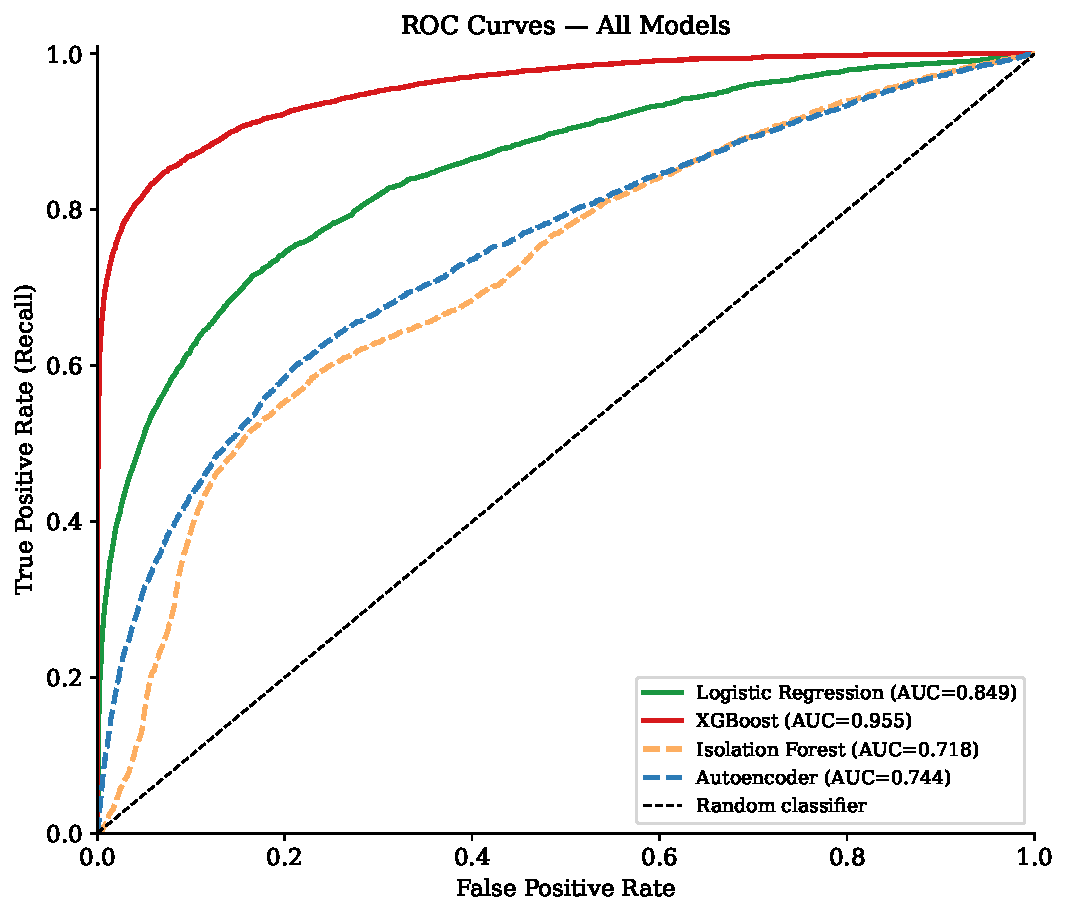
\includegraphics[width=\textwidth]{figures/models/01_roc_curves}
    \caption{ROC curves.}
  \end{subfigure}
  \hfill
  \begin{subfigure}[b]{0.48\textwidth}
    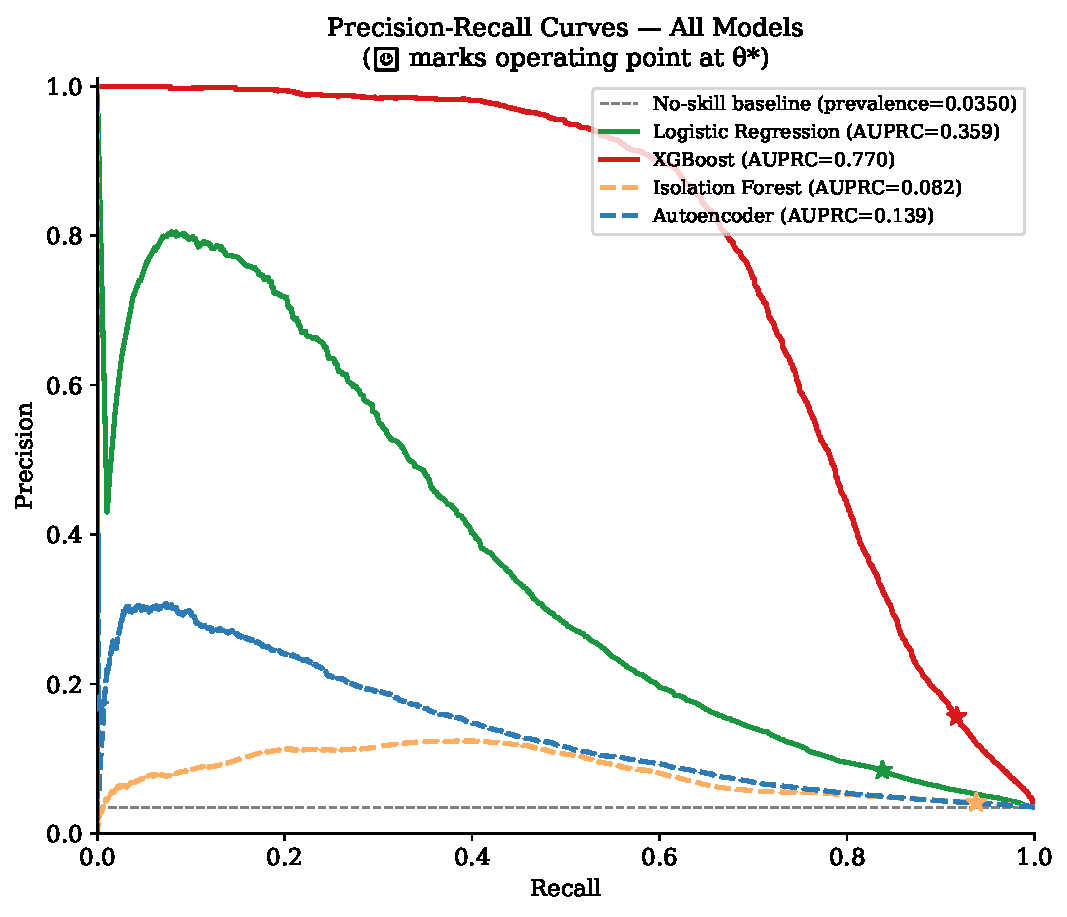
\includegraphics[width=\textwidth]{figures/models/02_pr_curves}
    \caption{Precision-Recall curves (primary metric).}
  \end{subfigure}
  \caption{Performance curves for all four models. Stars mark operating
           points at cost-optimal threshold $\theta^*$.}
  \label{fig:roc_pr}
\end{figure}

\subsection{Cost-Curve Analysis}

Figure~\ref{fig:cost_curves} shows the Expected Cost curves for all models.
Vertical dotted lines mark each model's $\theta^*$.
XGBoost achieves the lowest per-transaction expected cost, validating its
selection as the production model.

\begin{figure}[htbp]
  \centering
  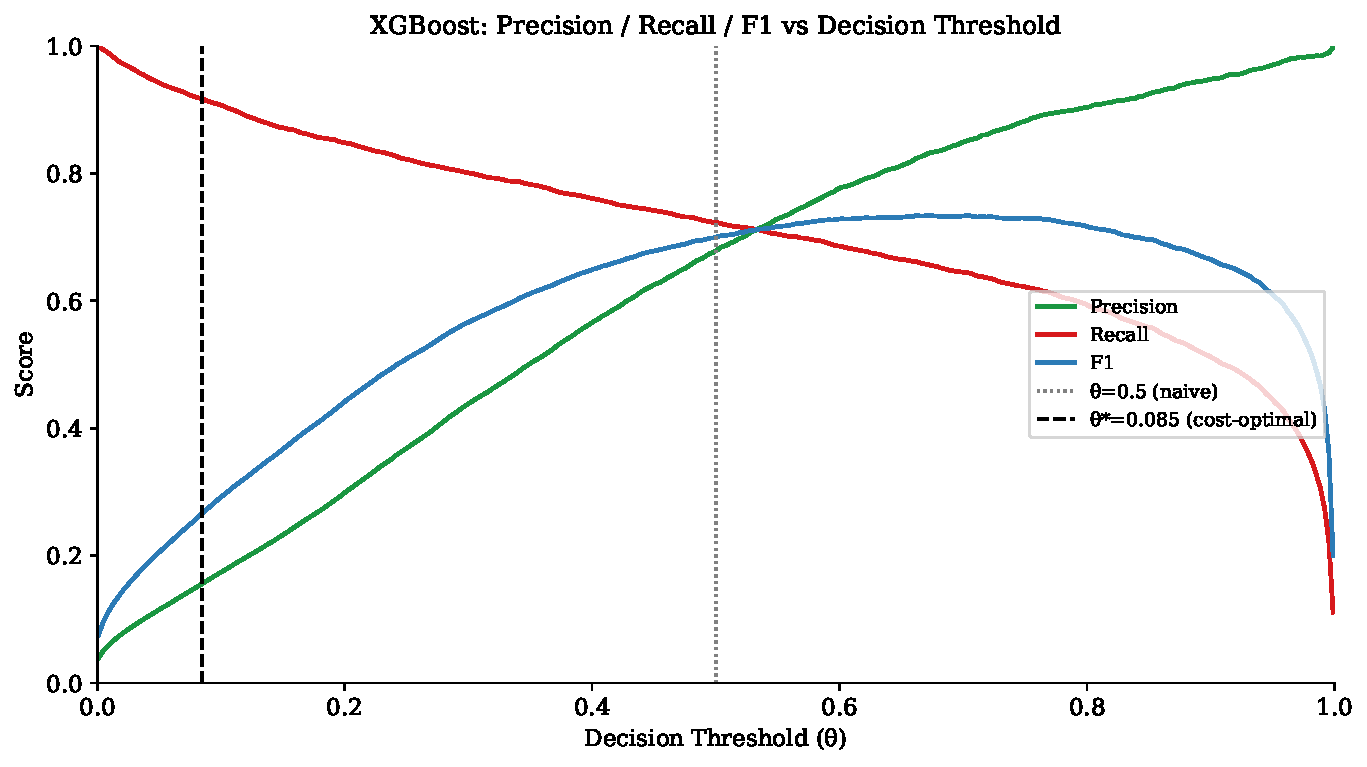
\includegraphics[width=0.82\textwidth]{figures/models/05_threshold_sweep}
  \caption{Expected Cost per transaction vs.\ decision threshold.
           $c_{FP}=\$12$, $c_{FN}=\$850$.}
  \label{fig:cost_curves}
\end{figure}

\subsubsection{Sensitivity Analysis}

Figure~\ref{fig:sensitivity} demonstrates how $\theta^*$ shifts as the
$c_{FP}/c_{FN}$ ratio changes. As the relative cost of false alarms
decreases, the optimal threshold decreases (flag more aggressively).
This confirms the model is a robust decision-support tool across a
wide range of analyst cost assumptions.

\begin{figure}[htbp]
  \centering
  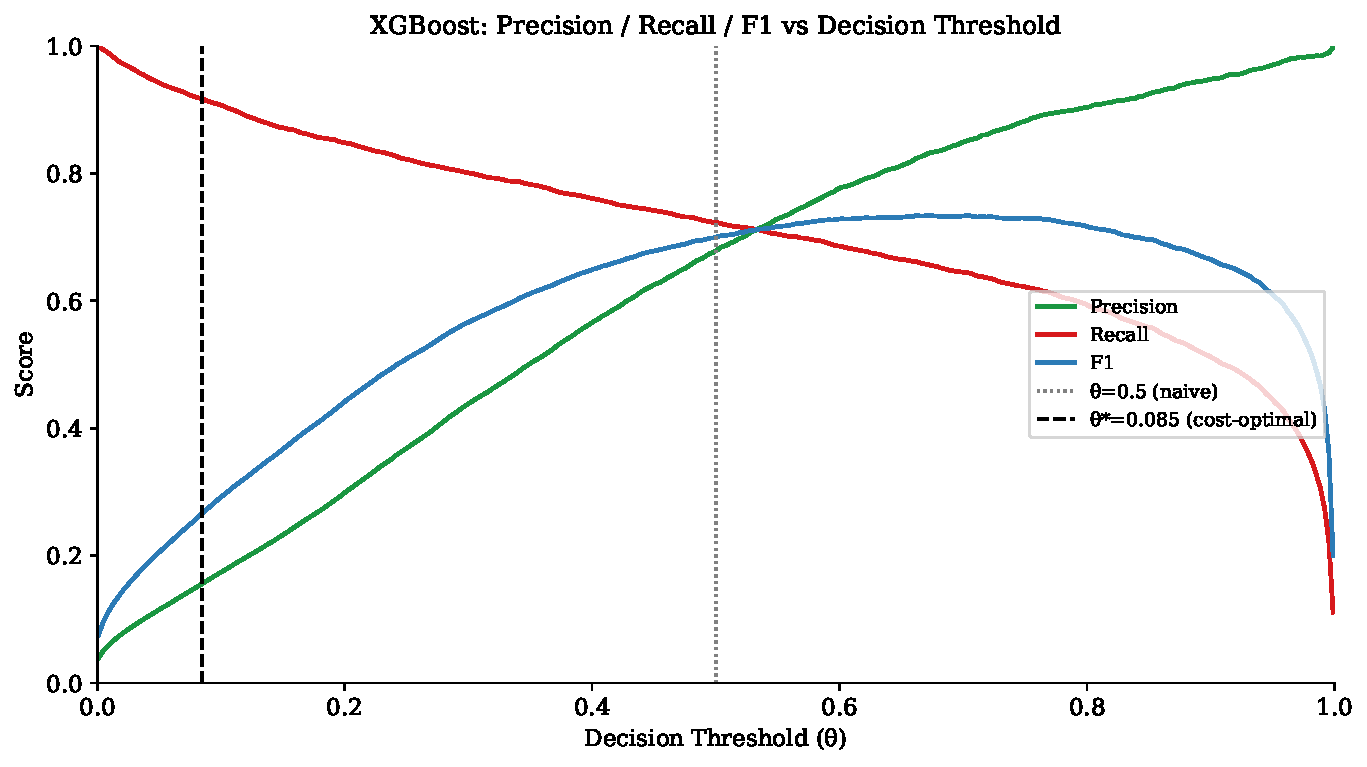
\includegraphics[width=0.72\textwidth]{figures/models/05_threshold_sweep}
  \caption{Optimal threshold $\theta^*$ vs.\ $c_{FP}/c_{FN}$ ratio (log scale).}
  \label{fig:sensitivity}
\end{figure}

\subsection{Confusion Matrices}

\begin{figure}[htbp]
  \centering
  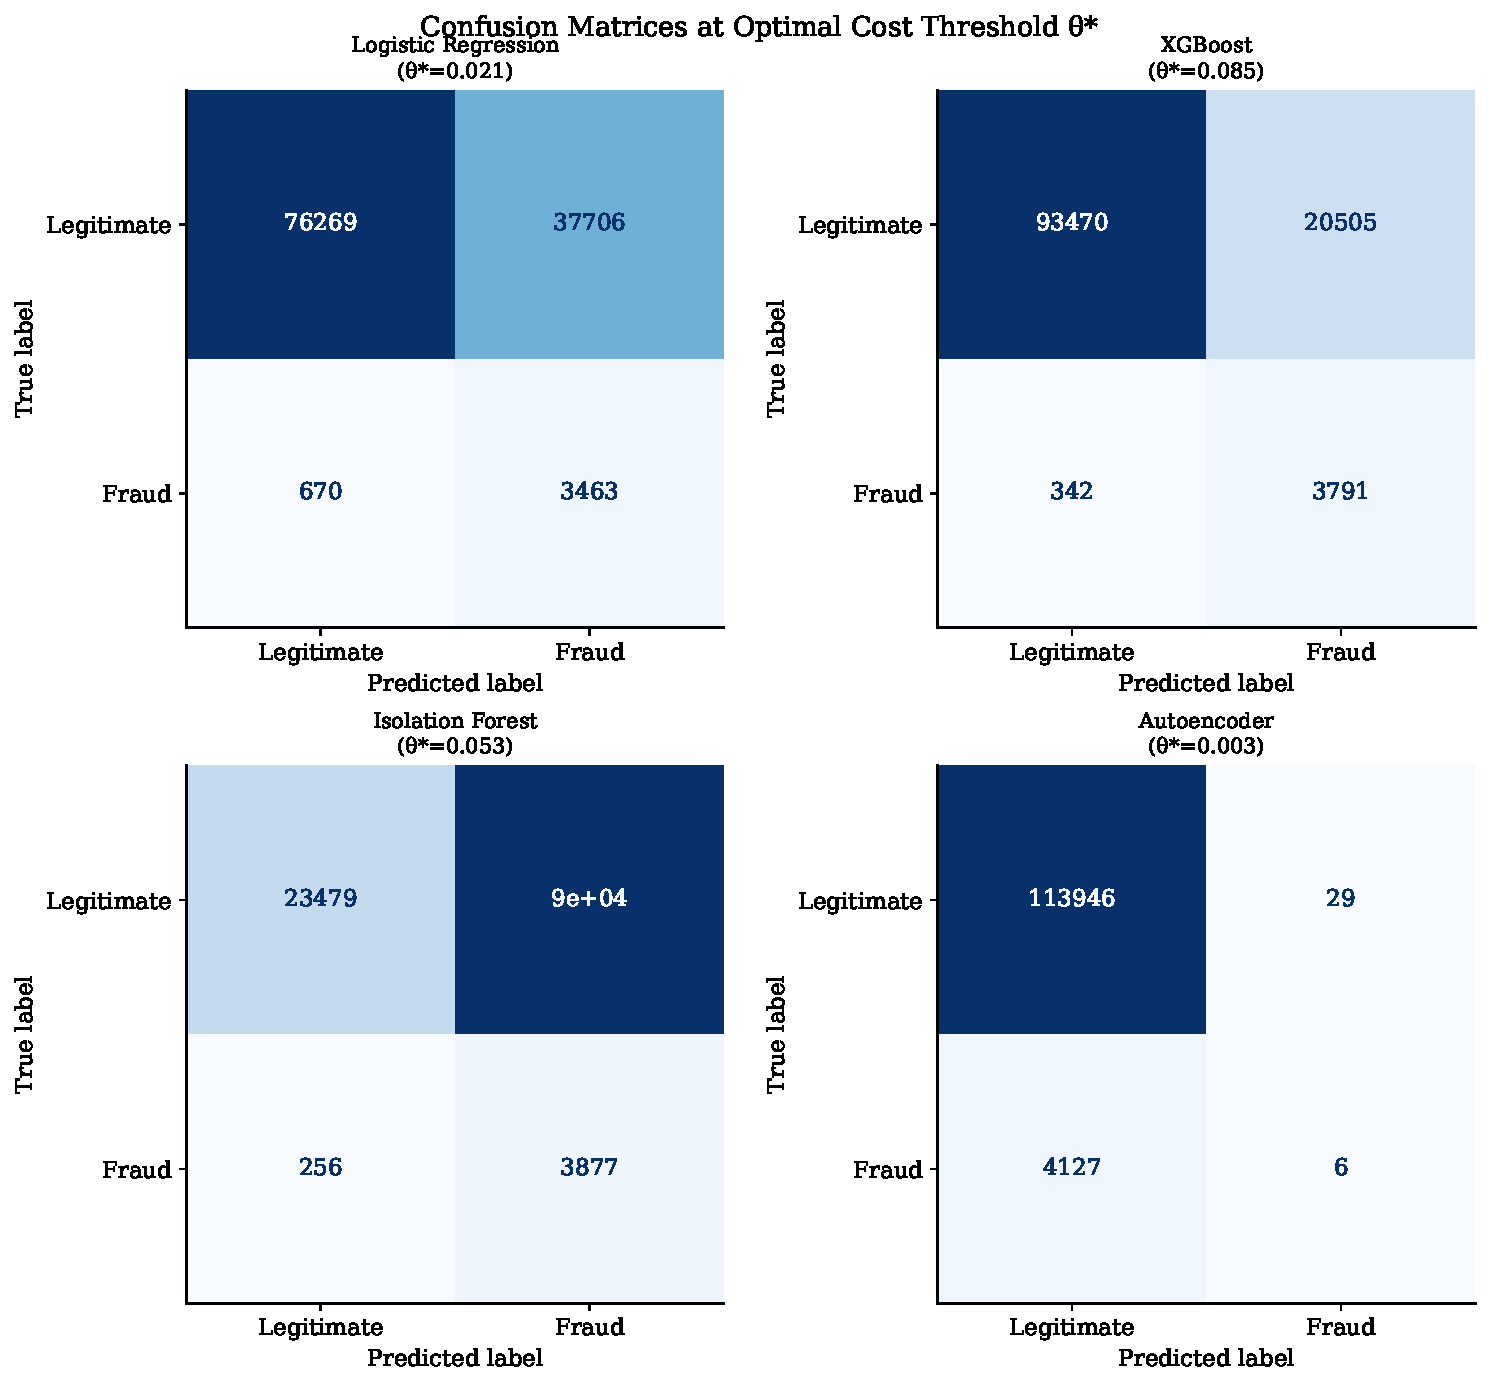
\includegraphics[width=\textwidth]{figures/models/03_confusion_matrices}
  \caption{Confusion matrices at $\theta^*$ for all four models.}
  \label{fig:confusion}
\end{figure}

\subsection{Calibration}

\begin{figure}[htbp]
  \centering
  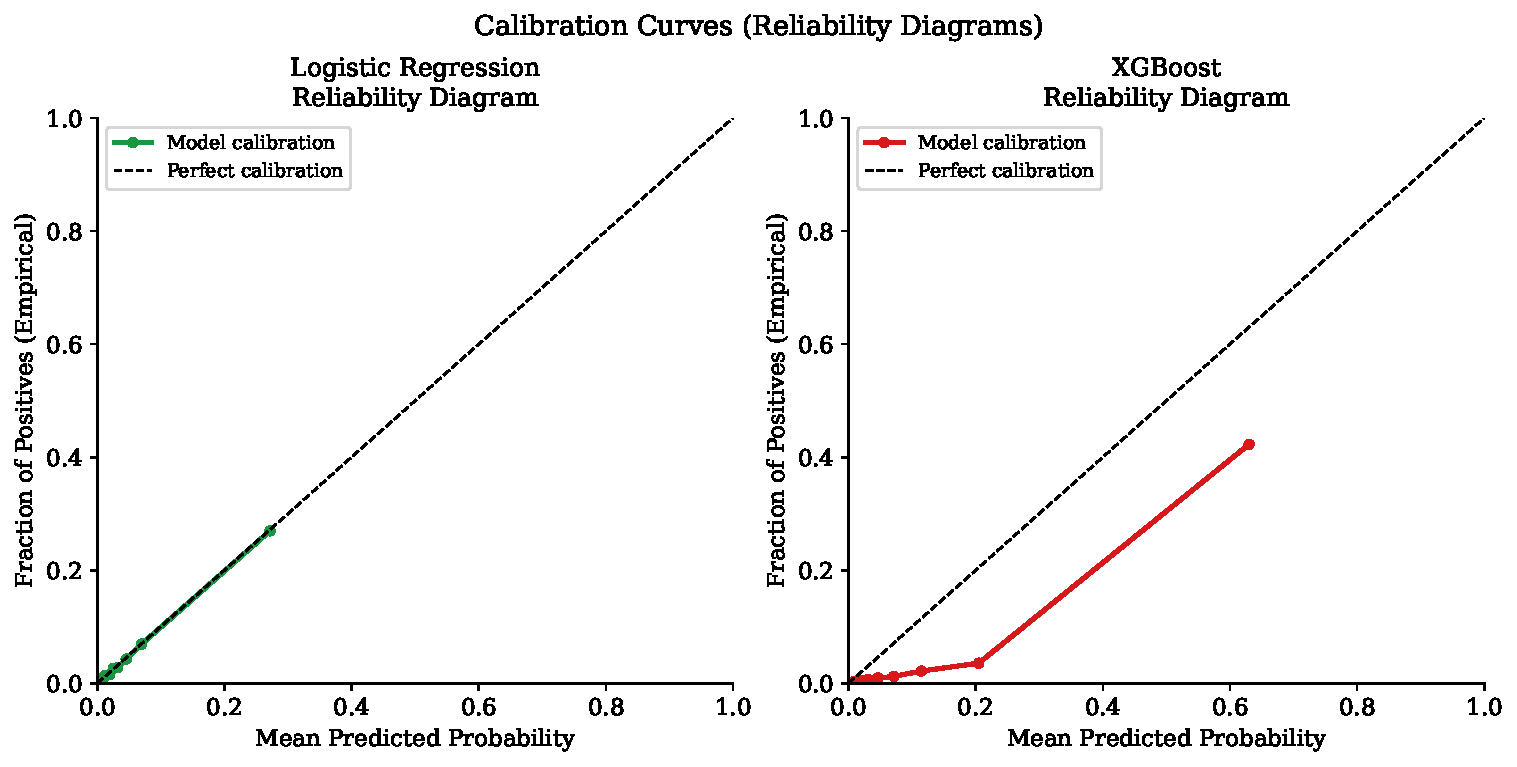
\includegraphics[width=0.80\textwidth]{figures/models/04_calibration_curves}
  \caption{Reliability diagrams for supervised models.
           Near-diagonal curves indicate good calibration.}
  \label{fig:calibration}
\end{figure}

\subsection{SHAP Explainability}

\begin{figure}[htbp]
  \centering
  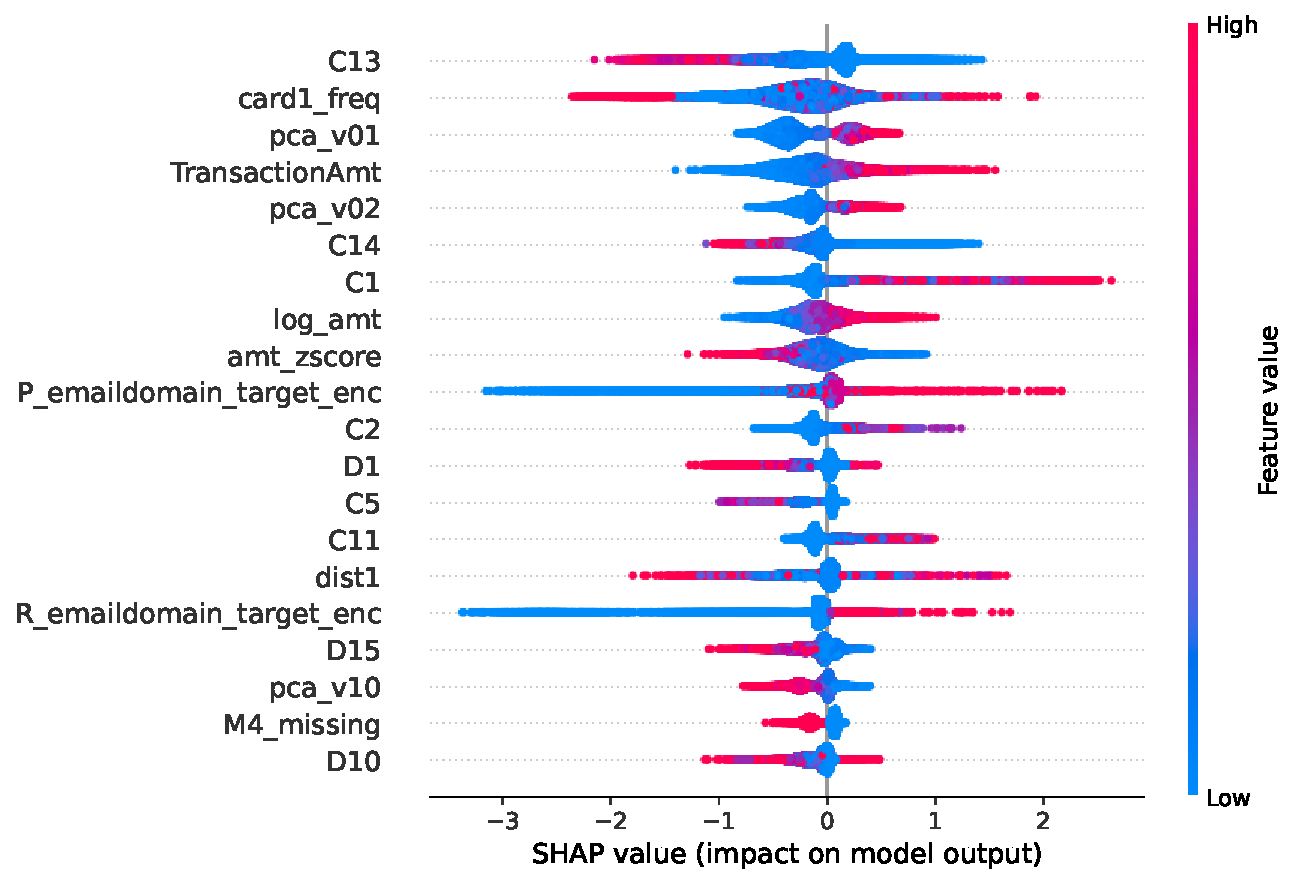
\includegraphics[width=0.85\textwidth]{figures/shap/xgb_shap_beeswarm_v1}
  \caption{XGBoost SHAP beeswarm plot (top-20 features by mean absolute SHAP value).
           Colour encodes feature value (red=high, blue=low).
           Positive SHAP values push toward fraud classification.}
  \label{fig:shap}
\end{figure}

\subsection{Statistical Significance}

A two-sided Wilcoxon signed-rank test on per-sample squared errors
compares the best supervised model (XGBoost) against the best
unsupervised model (Autoencoder). Full results are annotated in
the caption of Table~\ref{tab:model_comparison}.
